\chapter{Praxisteil}

\section{AP 2 - Elektronik}

\subsection{Anforderungen}

Bei der Elektronik gab es zwei verschiedene Bereiche: \\
In einem ersten Schritt sollte ein A-D Wandler gefunden werden, damit der vorhandene Drucksensor genauer ausgelesen werden kann. Zum Start es Projekts wurde der Drucksensor über das $\SI{10}{bit}$ breite analoge Interface des Arduino ausgelesen. Das ist für eine genaue Auswertung der Experimente zu wenig. Der Drucksensor hat einen Messbereich von (nachgucken) und gibt diesen auf $\SI{0}{} - \SI{10}{V}$ aus. Da der Arduino maximal $\SI{5}{V}$ als Eingangsspannung verarbeiten kann, wird die Spannung über einen Spannungsteiler auf $\SI{0} - \SI{5}{V}$ reduziert und dann eingelesen. Das entspricht einer Genauigkeit von $\SI{0,004}{V/bit}$, was einer Genauigkeit von XXX mbar/Volt entspricht. \\
\hfill \\
Als Resultat soll die gesamte Elektronik als \glqq Blackbox\grqq \ vorliegen, sodass man nach außen hin nur noch Anschlüsse hat, die klar gekennzeichnet sind. Dies soll in Form eines Gehäuses erledigt werden, das zudem auch noch rudimentären Schutz gegen Schmutz bietet.


\subsection{Umsetzung}

\subsubsection{Elektronik}

Der Arduino bietet einen sehr einfachen SPI Bus zum Anschluss von Modulen an. Darüber können die digitalen Outputdaten, der angesteckten Module ausgelesen werden, unabhängig davon wie hoch die Auflösung der Module ist. Auf Grund dieser Voraussetzungen wurde entschieden ein Modul für diesen Bus zu verwenden. \\
Rechnung für 16 bit einfügen!!!!!! \\
Es gibt verschiedene $\SI{16}{bit}$ A-D Wandler auf dem Markt, allerdings gibt es den hier ausgewählten (einfügen!!!!) bereits auf einer fertig montierten Platine, die direkt in den Arduino eingesteckt werden kann. Zudem gibt es zu der Platine eine recht gute Dokumentation. 


Schaltskizze!!!

\subsubsection{Gehäuse}

Da es insbesondere im Lichtstreuaufbau nur sehr begrenzten Stauraum gibt und sämtliche Bauteile, das Wirbelbett selbst ausgenommen, auf einer Platte verbaut werden sollen, wurde gegen ein kommerziell erhältliches Gehäuse entschieden. \\ 
Stattdessen wurde ein Gehäuse entworfen, in dem sowohl der Arduino als auch das Board mit der Schaltung passgenau Platz finden. Dabei wurde darauf geachtet, dass die Kontakte unterhalb des Arduinos und des Boards genug Platz haben, sodass es keinerlei unbeabsichtigte Reibung der Komponenten am Gehäuse gibt. \\
Für die Anschlüsse wurden möglichst kleine Löcher im Gehäuse gelassen, sodass ein größtmöglicher Schutz gegen Schmutz bei größtmöglichem Komfort gewährleistet wird. \\
Um die Komplexität so gering wie möglich zu halten, wurde sich gegen einen Schließmechanismus entschieden, da dieser entweder anfällig oder unnötig teuer werden würde. Da das Gehäuse lediglich zum entfernen der angeschlossenen Kabel geöffnet werden muss, war es am einfachsten, den Deckel mit Klebeband am Gehäuse fest zu machen.

Hier Bilder einfügen!!


\section{AP3 - Gassystem}

\subsection{Anforderungen (kommt das hier hin?)}

Die Aufgabe bestand darin, trotz der Integration des Luftbefeuchters, das Gassystem als Einheit so kompakt und stabil wie möglich zu gestalten. Es sollte zusammen mit der Elektronik zusammen in den Lichtstreuaufbau passen und dort die Rotationbewegung des Aufbaus nicht einschränken.


\subsection{Umsetzung}

\subsubsection{Flowcontroller}

Um die Anforderung der Erweiterung des Regelbereichs beim Gasstrom auf $\SI{0} - \SI{3000}{l/h}$ zu erfüllen, musste der bisherige Flowcontroller mit einem Regelbereich von $\SI{0} - \SI{120}{l/h}$ ersetzt werden. \\
Die Idee einer konstruktiven Lösung den Strom über mehrere Gasdurchflussbegrenzer und Ventile auf definierte Werte voreinzustellen und mit dem vorhandenen Flowcontroller von da ab zu regeln, wurde verworfen, weil es sich als zu ungenau und nicht deutlich billiger in Aufwand und Kosten darstellte. \\
Die Lösung bestand darin einen neuen Flowcontroller anzuschaffen, der den gesamten Regelbereich mit einer hinreichenden Genauigkeit abdeckt und gleichzeitig gut in das Gassystem integriert werden kann. Dazu wurden Angebote eingeholt, die im folgenden dargelegt sind:

\begin{tabular}{|c|c|c|}
	\hline  & Brooks & Bronkhorst \\ 
	\hline Regelbereich & $\SI{0} - \SI{3000}{l/h}$ & $\SI{0} - \SI{3000}{l/h}$ \\ 
	\hline Genauigkeit $20 - \SI{100}{\%}$ & $\pm \SI{0,9}{\%}$ & $\pm \SI{0,5}{\%}$ Istwert $+ \pm \SI{0,1}{\%}$ Endwert\\ 
	\hline Genauigkeit $0 - \SI{20}{\%}$ & $\pm \SI{0,18}{\%}$ & $\pm \SI{0,5}{\%}$ Istwert $+ \pm \SI{0,1}{\%}$ Endwert \\ 
	\hline Preis in \euro & 1187,33 & 1382,66 \\ 
	\hline 
\end{tabular} 

\vspace{0,5cm}

Es wurde sich für den Flowcontroller der Firma Brooks entschieden. Das geschah aus mehreren Gründen: \\
Im ursprünglichen Aufbau war auch ein Flowcontroler von Brooks verbaut, daher wussten wir wie dieser angesteuert wird und hatten bereits den benötigten Stecker. Weiterhin ist die Genauigkeit des Brookscontrollers im niedriegen Regelbereich besser als die des Bronkhorstcontrollers. Dies ist grade bei quantitativen Messungen mit kleinen Rohrdurchmessern und sehr feinen granularen Medien essentiell. \\
Zudem waren die Anschaffungskosten für den Brookscontroller um ca $\SI{200}{Euro}$ niedriger.\\
Außerdem hatte die Gruppe bei einem anderen Controller von Bronkhorst einige Probleme mit der Zuverlässigkeit gehabt, während der Brooks Controller keine aufwies.


\subsubsection{Verrohrung}

Eine Herstellerauswahl hat hier nicht stattgefunden, da bereits vorhandene Verrohrung weitergenutzt werden sollte, deshalb wurde weiterhin auf Swagelok gesetzt. Dies hatte auch den Vorteil, das ein Berater aus dem nahegelegenen Standort Düsseldorf bei der Auslegung und Wahl der Komponenten beraten konnte. \\
Auf der Skizze in Abbildung xy kann man das gebaute System sehen:
\hfill \\

Skizze Einfügen


Bei der Verrohrung wurde sich für eine Kombination aus Edelstahlrohren und Bunaschläuchen entschieden. Dies bietet dem System die nötige Flexibilität im Bezug auf Anschluss an das Wirbelbett und die Luftzufuhr, als auch die nötige Robustheit und Stabilität. Sämtliche Rohrleitungen vom Druckminderer bis zum Übergang zum Wirbelbett sind aus Edelstahl. \\
Die Ventile, T-Stücke und Verbindungsstücke sind auch aus Edelstahl, da Messing zwar billiger wäre, allerdings auch weicher, was zu Verformungen und höherem Verschleiß führen kann.


\subsubsection{Luftbefeuchter}

Für den Luftbefeuchter wurden drei unterschiedliche Lösungen geprüft:

\paragraph{Swagelok} 

\hfill \\

Von Swagelok gibt es eine Lösung ähnlich dem jetzigen Drucksensor. Über ein spezielles Rohrverbindungsstück kann ein Metallzylinder angeschlossen werden, der Senkrecht in auf dem Rohr nach oben steht. Dieser wird mit Wasser gefüllt, das von unten mit Luft durchströmt wird und anschließend oben abgenommen und Richtung Wirbelbett fließt.

\paragraph{Befeuchtung durch Vorbeiströmen}

\hfill \\

In einer anderen Arbeit (hier quelle einfügen) wurde die Luftbefeuchtung realisiert, oindem man Luft direkt an einer  WasserOberfläche vorbeiströmen ließ und die Luft durch Diffusion Wasser aufnahm. 

\paragraph{Befeuchtung durch Durchströmen}
\hfill \\

Die einfachste Methode Luft zu befeuchten, ist sie durch ein Wasserbad zu leiten und sie anschließend geeignet abzugreifen.


\paragraph{Auswahl}

\hfill \\

Es wurde sich für die Methode \glqq Befeuchtung durch Durchströmen\grqq \ entschieden, da die anderen Methoden Mängel aufweisen. Die Lösung von Swagelok ist zum einen sehr teuer, zudem würde bei angeschaltetem Gasfluss Wasser in das System fließen. \\
Die Methode des Vorbeiströmens fiel raus, weil eine zu große Strömfläche gebraucht wurde. Anhand der Formeln aus der Arbeit von Herrn Schmitz, erhielt man eine Fläche von $\SI{50}{cm} \cdot \SI{50}{cm}$. Ein Aufbau dieser Größe ist unmöglich im Lichtstreuaufbau unterzubringen.

\paragraph{Umsetzung}

\hfill \\

Ursprünglich sollte der Luftbefeuchter so ausgelegt werden, sodass der gesamte Regelbereich des Controllers abgedeckt ist. In Versuchen hat sich allerdings gezeigt, das dafür ein Wasservolumen von $7 - \SI{8}{l} $ nötig wäre. Eine Aperatur dieser Größe wäre schwer bis unmöglich im Lichtstreuaufbau unterzubringen. Daher wurde ein Behältnis, das in den Aufbau passt, gewählt und damit ist nun ein Flussbereich von $0 - \SI{000000000}{l/h}$ abdeckbar. \\
Eine weitere Herausforderung war die Luft mit dem geforderten Feuchtigkeitsgrad von $\SI{75}{\%}$ anzureichern. \\

Skizze einfügen!!!!

Ein erprobtes Verfahren ist, die Luft durch eine gesättigte Kochsalzlösung zu leiten. Dadurch wird automatisch eine Luftfeuchtigkeit von $\SI{75}{\%}$ erreicht. Die Luft muss allerdings als sehr feine Blasen durch die Kochsalzlösung wandern, da die Steigzeit sonst nicht ausreicht die Luft anzureichern. \\
Dies wurde erreicht indem die Luft aus einer Schlauchspirale mit feinen Löchern durch eine zweilagige Schicht aus handelsüblichen Küchenschwämmen geleitet wurde. \\
Damit die Schwämme nicht durch den Luftstrom von ihrem Platz weggedrückt werden, wurde in $\SI{2}{cm}$ darüber ein Netz gespannt.



\section{AP4 - Wirbelbett}


\subsection{Überblick}

Da das bisherige Wirbelbett nicht flexibel genug konfigurierbar war, musste es möglichst modular neu konstruiert werden. Es wurde daher entschieden das Wirbelbett aus 4 Teilen plus dem Probenröhrchen zu bauen. Die einzelnen Teile sind:

\begin{itemize}
	\item Anschlusszylinder
	\item unterer Röhrchenhalter
	\item oberer Röhrchenhalter
	\item Trichter
\end{itemize}


Hier Bild einfügen!!!!


Die Komponenten werden im folgenden beschrieben.


\subsection{Methode zum Granulat auffangen}

\subsubsection{Anforderung}

Wie schon in der Einleitung beschrieben, hat granulares Medium gleichzeitig mehrere Phasen, von denen die oberste die Gasphase ist. Je nach Füllstand und Gasfluss des Messröhrchens kann es nun passieren, das einzelne Partikel oben aus dem Röhrchen hinausfliegen. Dies gilt es zu verhindern.

\subsubsection{Auswahl}

\paragraph{Fliehkraftabscheider} 

\hfill \\

Ein sehr beliebtes Produkt, um Luft von Partikeln zu säubern, ist der Fliehkraftabscheider oder Zyklon. Dieser basiert auf dem Prinzip, das die Luft immer weiter beschleunigt wird und die darin enthaltenen Partikel an die Wand gedrückt werden und schließlich nach unten raus fallen. \\


\begin{figure}[h]
	\begin{center}
		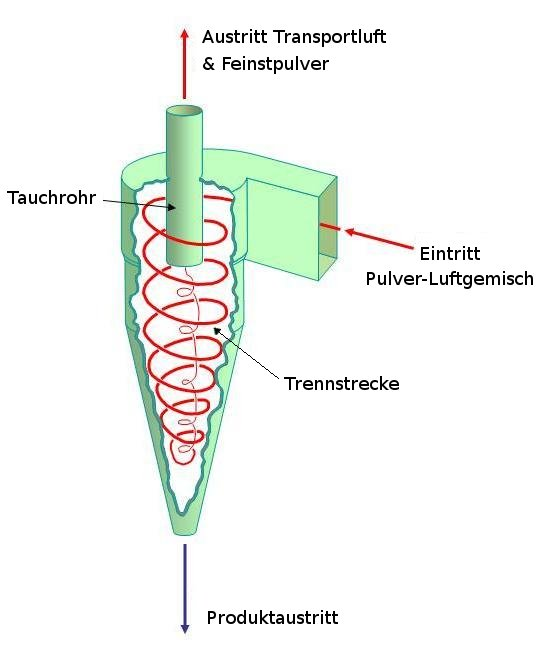
\includegraphics[scale=0.4]{Umsetzung_Fliehkraftabscheider.jpg}
		\caption{Fliehkraftabscheider: Quelle Wikipedia}
	\end{center}
\end{figure}



Das Problem bei diesem Bauteil besteht darin, das die kommerziell erhältlichen Versionen sehr teuer sind und zudem zu groß für unserem Aufbau passen. \\
Weiterhin wäre ein erheblicher Konstruktionsaufwand nötig, um einen eigenen Zyklon zu bauen, da die Luft in unserem Versuch von unten kommt, der Zyklon sie aber von der Seite braucht. \\
Aus diesem Grund haben wir uns für das im folgenden beschriebene Prinzip entschieden.


\paragraph{Erweiterung des Querschnitts}

\hfill \\

Wie man anhand der Formel $v_a = \frac{Q}{A}$ \cite{Grollius2012} sehen kann, ist die Geschwindigkeit des Gasstrom direkt proportional zum Querschnitt des Rohrs. Wenn man also den Querschnitt verdoppelt, dann viertelt man die Geschwindigkeit des Gasstroms. 


\subsubsection{Umsetzung}

Um den Gasstrom zu verlangsamen und gleichzeitig das Einfüllen des Granulats zu erleichtern, wurde jeweils ein Trichter konstruiert, der passgenau mit dem Innendurchmesser jedes Probenröhrchens abschließt und zudem den Querschnitt verdoppelt. \\
Zudem wurde ein abnehmbarer Filter oben auf den Trichter gespannt, um einen rudimentären Schutz gegen austretende Partikel bei Fehlbedienung zu gewährleisten.





